\section{Durchführung}
\label{sec:Durchfuehrung}
\subsection{Charakteristische Strahlung von Kupfer}
Zu Beginn des Versuchs sollen mithilfe des Kupfer Spektrums die Energien der $K_{\alpha}$ und $K_{\beta}$ Schale bestimmt werden.
Dafür werden die Elektronen mit 35keV auf die Anode aus Kupfer beschleunigt, die entstandene Strahlung wird auf einen LiF-Kristall gelenkt.
Im Versuchsaufbau lässt sich der LiF Kristall über ein Winkelintervall von 8° bis 25° drehen und die emittierte Strahlungsintensität kann gemessen werden.
Dabei wird die Bragg Reflexion ausgenutzt und die Winkel können einer entsprechenden Wellenlänge zugeordnet werden(Gl. \ref{eqn:Bragg_Gleichung}).

\subsection{Wellenlängenabhängigkeit der Transmission}
Um im weiteren Versuchsverlauf die Compotonwellenlänge zu bestimmen muss zunächst der Zusammenhang zwischen Transmission und Wellenlänge bestimmt werden.
Der Versuch wird wieder gleich aufgebaut, allerdings wird nun eine Aluminium Platte hinzugefügt.
Der LiF Kristall wird diesmal von 7° bis 10° in 0,1° Schritten gedreht und die Impulsrate wird jeweils über 200s gemessen.
Dieselbe Messung wird nochmal ohne Aluminium Absorber wiederholt.

\subsection{Compton Wellenlänge}
Für die Messung der Compton Wellenlänge wird der LiF-Kristall durch eine Plexiglasscheibe erstzt, in der die Compton Streuung stattfinden kann. Um nur um 90° gestreute Photonen zu messen wird das Zählrohr im entsprechenden Winkel platziert (Abb. \ref{fig:Exp_Aufbau_2}).
Nun wird einmal die Zählrate ohne jeglichen Absorber gemessen, einmal wird der Absorber zwischen Quelle und Plexiglas und einmal zwischen Plexiglas und Zählrohr platziert.
In diesem Versuchsteil wird über 300s gemessen.
\begin{figure}
    \centering
    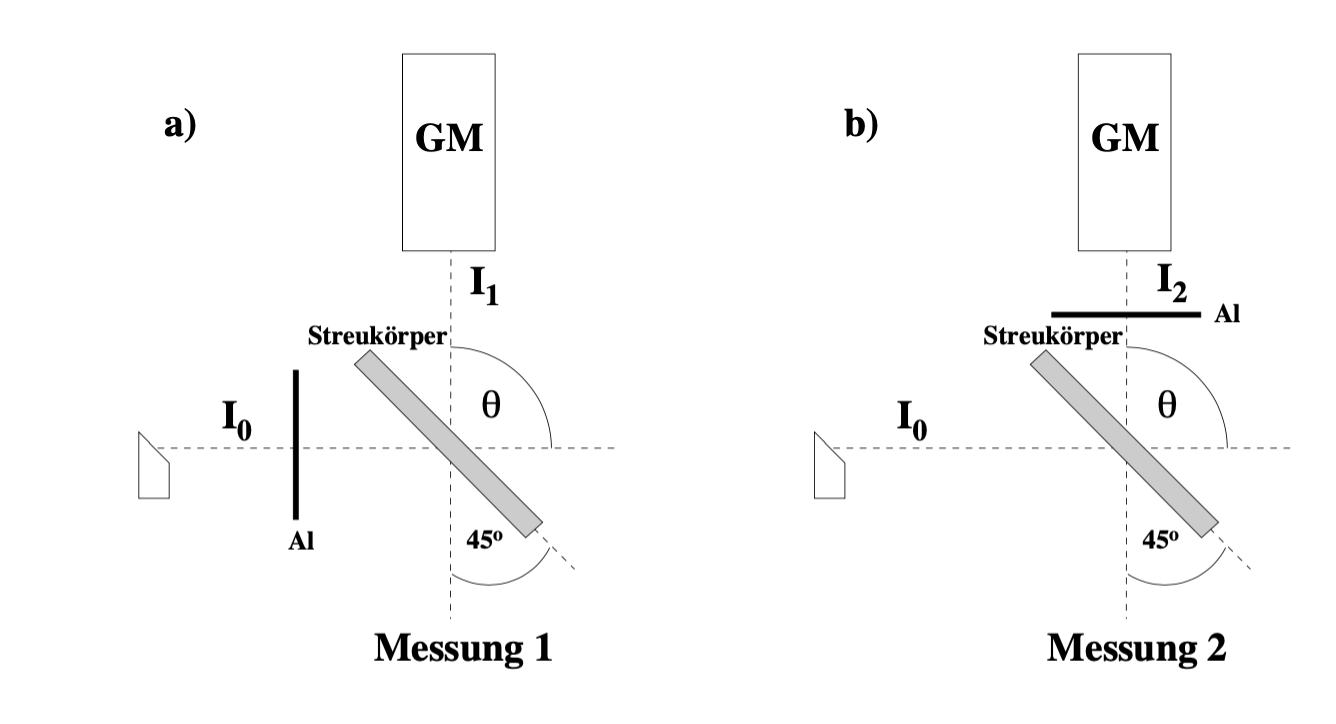
\includegraphics[width=0.7\textwidth]{bilder/Exp_Aufbau_2.png}
    \label{fig:Exp_Aufbau_2}
    \caption{Versuchsaufbau zur Messung der Compton Wellenlänge}
\end{figure}
